% !TeX program = xelatex
% !TeX encoding = UTF-8 Unicode
% !BIB program = biber

% essa classe aceita as seguintes opções:
% abnd ou ieee pra estilo de citaçõ
% english ou french pra língua dos slides (não passar nada é português)
\documentclass[abnt]{slides}

\title{Inteligência Computacional - Atividade Prática 01}
\subtitle{Análise e Pré-processamento de Dados (Adult Census Income)}

% Todo comando \add trabalha com uma lista e todo comando \set trabalha com um
% único elemento, ou seja, pode haver apenas um \setorientador mas vários
% \addauthor ou \addcoorientador. Todo comando \add e \set tem um \get
% correspondente (por exemplo, \getauthors, \getcoorientadores, \getorientador,
% \getmembrobanca). Esses comandos são definidos na classe slides.cls. No caso
% dos \set, os \get são implicitos, e não você não vai encontrá-los na classe.

\addauthor{João Paulo da Cunha Faria}{joaopaulo@example.com}
\setorientador{Prof.\ Dr.\ Alisson Marques da Silva}
\addcoorientador{Não se aplica}

\setdepartamento{Engenharia de Computação}
\setlocal{CEFET-MG}
\setano{2026}

\preamble{}

% Essa classe usa o biblatex com backend biber ao invés do bibtex.
\addbibresource{bibliothek.bib}

% Controla o texto das captions das figuras. Neste caso, centraliza.
\captionsetup{justification=centering}

\begin{document}
\maketitle{}

% Eu gosto de separar meus documentos \latex em vários arquivos, para manter
% organizado.
% !TeX root = document.tex
% !TeX encoding = UTF-8 Unicode

\section{Introdução e Análise Exploratória}

\begin{slide}{Objetivo do Trabalho}
  \begin{itemize}
    \item Desenvolver um experimento contemplando análise e compreensão dos dados.
    \item Aplicar pré-processamento e definir uma metodologia experimental adequada.
    \item Comparar modelos de forma reprodutível e metodologicamente correta.
  \end{itemize}
\end{slide}

\begin{slide}{Contextualização do Problema}
  \begin{itemize}
    \item \textbf{Descrição:} identificação do problema associado ao conjunto de dados.
    \item \textbf{Cenário:} predição de renda anual com dados do censo de 1994.
    \item \textbf{Objetivo do modelo:} prever se a renda anual supera 50 mil dólares.
    \item \textbf{Tipo de tarefa:} classificação binária.
  \end{itemize}
\end{slide}

\begin{slide}{Caracterização Geral da Base}
  \begin{itemize}
    \item \textbf{Fonte:} UCI Machine Learning Repository.
    \item \textbf{Total de instâncias:} 32.561 registros.
    \item \textbf{Número de atributos:} 14 variáveis preditoras.
    \item \textbf{Atributos mistos:} variáveis categóricas, inteiras e reais.
  \end{itemize}

  \vspace{0.3cm}
  \scriptsize
  \begin{table}
    \centering
    \begin{tabular}{llll}
      \toprule
      age & workclass & fnlwgt & education \\
      education-num & marital-status & occupation & relationship \\
      race & sex & capital-gain & capital-loss \\
      hours-per-week & native-country &  &  \\
      \bottomrule
    \end{tabular}
    \caption{Lista de atributos da base Adult Census Income.}
  \end{table}
\end{slide}

\begin{slide}{EDA: Distribuição de Idade}
  \begin{itemize}
    \item \textbf{Método:} histogramas para visualizar concentração dos dados.
    \item \textbf{Observação:} maior parte da amostra entre 20 e 50 anos.
    \item \textbf{Importância:} compreender a demografia e reduzir vieses geracionais.
  \end{itemize}

  \begin{figure}
    \centering
    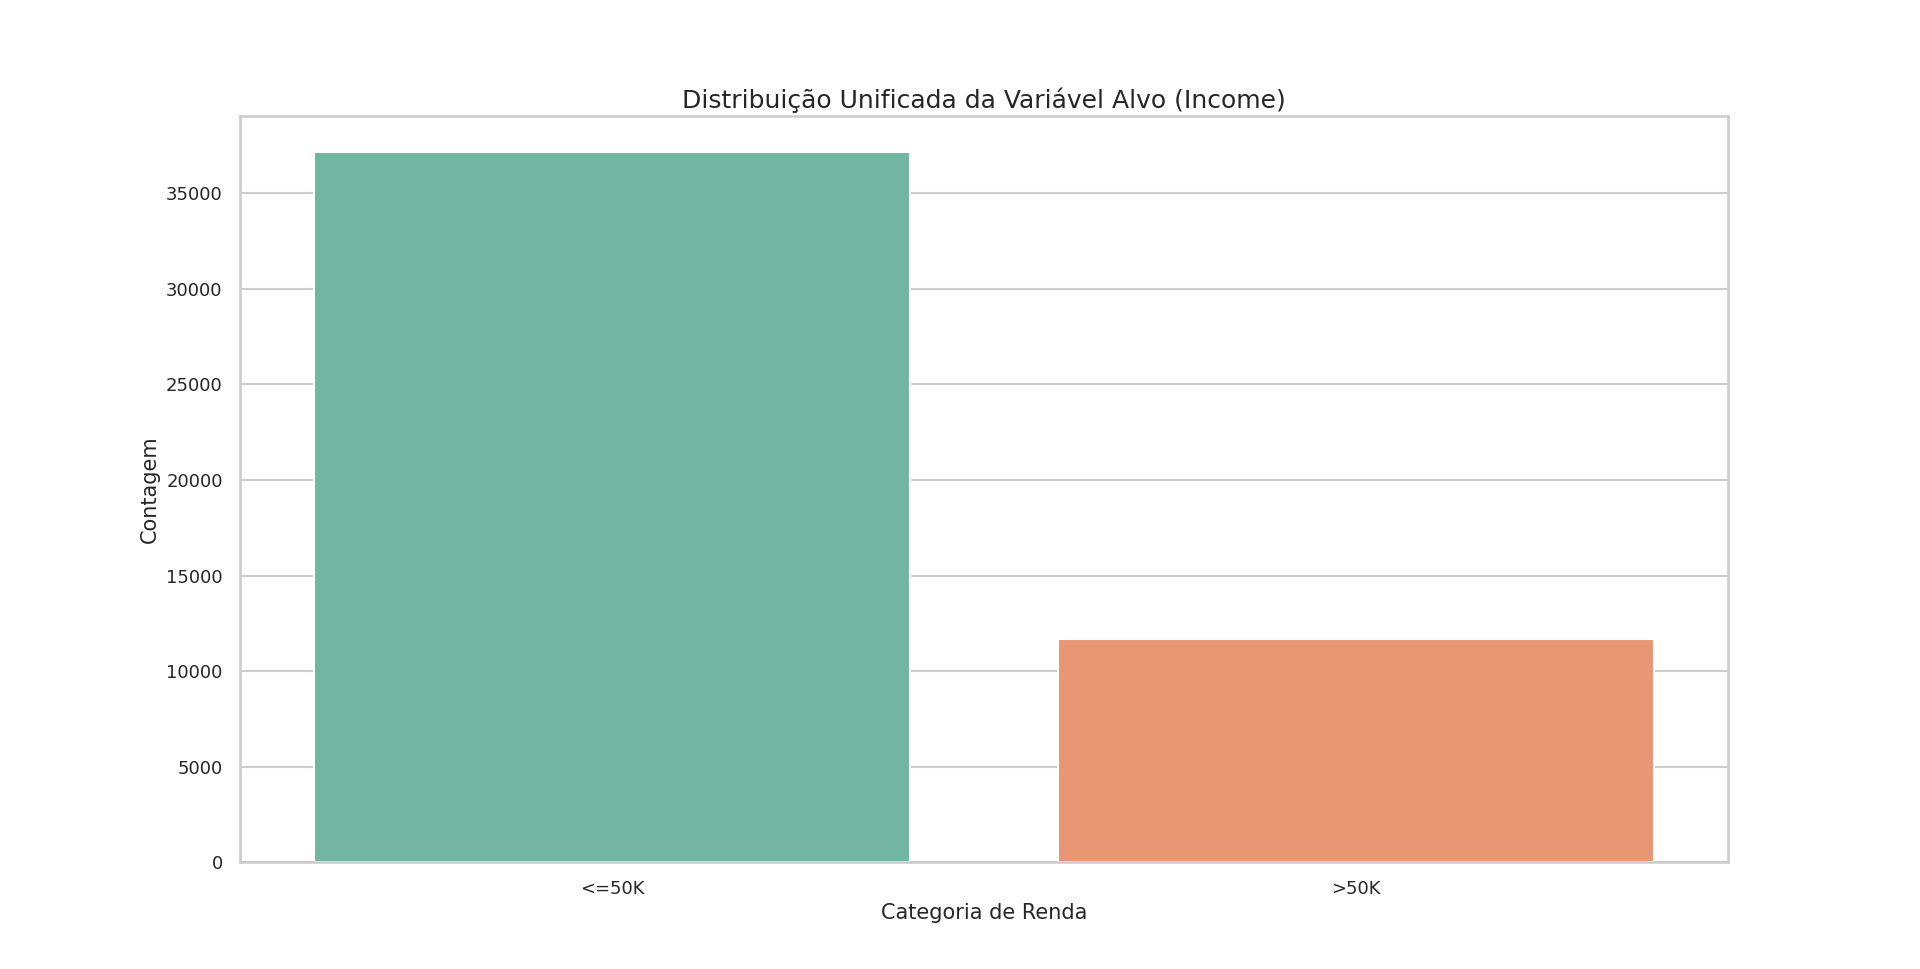
\includegraphics[width=0.72\textwidth]{../atividade_1/images/histograma.png}
    \caption{Histograma da variável idade.}
  \end{figure}
\end{slide}

\begin{slide}{EDA: Horas Trabalhadas e Renda}
  \begin{itemize}
    \item \textbf{Método:} boxplots relacionando horas semanais e classe de renda.
    \item \textbf{Outliers:} casos extremos de até 99 horas por semana.
    \item \textbf{Tendência:} renda \textgreater 50K tende a maior carga horária média.
  \end{itemize}

  \begin{figure}
    \centering
    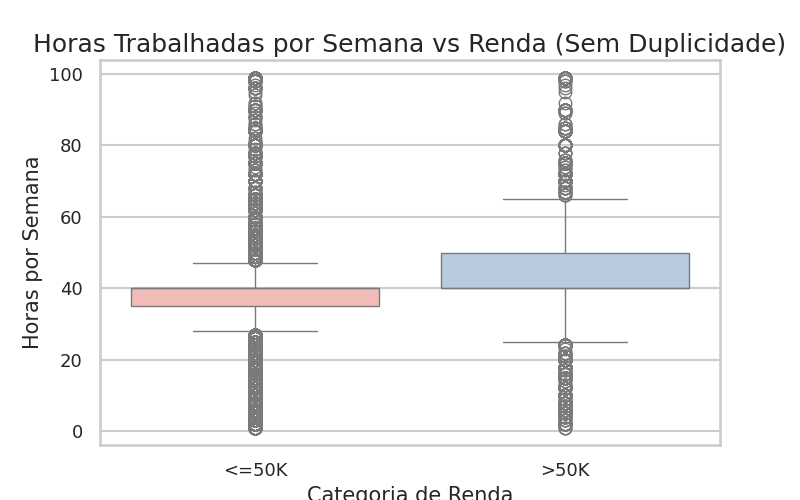
\includegraphics[width=0.72\textwidth]{../atividade_1/images/boxplot.png}
    \caption{Distribuição de horas por semana por classe de renda.}
  \end{figure}
\end{slide}

\begin{slide}{Identificação de Problemas de Qualidade}
  \begin{itemize}
    \item \textbf{Valores ausentes:} presença de ``?'' em colunas como workclass e occupation.
    \item \textbf{Ruídos de rótulo:} inconsistência entre ``\textless=50K'' e ``\textless=50K.''.
    \item \textbf{Desbalanceamento:} classe de menor renda representa aproximadamente 76\%.
    \item \textbf{Redundância:} atributo education redundante em relação ao education-num.
  \end{itemize}
\end{slide}

% !TeX root = document.tex
% !TeX encoding = UTF-8 Unicode

\section{Pré-processamento e Metodologia}

\begin{slide}{Pré-processamento: Limpeza e Seleção}
  \begin{itemize}
    \item \textbf{Tratamento de ausentes:} imputação pela moda para variáveis categóricas.
    \item \textbf{Seleção de atributos:} remoção de fnlwgt por baixa relevância para predição individual.
    \item \textbf{Redução de redundância:} descarte da coluna education, mantendo education-num.
  \end{itemize}
\end{slide}

\begin{slide}{Pré-processamento: Transformação de Dados}
  \begin{itemize}
    \item \textbf{Codificação:} One-Hot Encoding para variáveis nominais.
    \item \textbf{Justificativa:} evita hierarquia artificial entre categorias nominais.
    \item \textbf{Normalização:} StandardScaler para padronizar escala dos atributos numéricos.
  \end{itemize}
\end{slide}

\begin{slide}{Metodologia Experimental}
  \begin{itemize}
    \item \textbf{Estratégia de divisão:} hold-out com 80\% para treino e 20\% para teste.
    \item \textbf{Estratificação:} manutenção da proporção das classes em treino e teste.
    \item \textbf{Justificativa:} avaliação justa, simples e reprodutível.
  \end{itemize}
\end{slide}

\begin{slide}{Algoritmos Selecionados}
  \begin{itemize}
    \item \textbf{Random Forest:} robusto para alta dimensionalidade após o encoding.
    \item \textbf{Regressão Logística:} baseline estatístico para comparação.
    \item \textbf{KNN (k=5):} avalia impacto da esparsidade no espaço de atributos.
  \end{itemize}
\end{slide}

\begin{slide}{Discussão: Por que o F1-Score?}
  \begin{itemize}
    \item \textbf{Problema:} em bases desbalanceadas, acurácia pode ser enganosa.
    \item \textbf{Solução:} F1-Score equilibra Precisão e Recall.
    \item \textbf{Objetivo:} melhorar a identificação da classe minoritária (\textgreater 50K).
  \end{itemize}

  \[
    F_1 = 2 \cdot \frac{\text{Precisão} \cdot \text{Recall}}{\text{Precisão} + \text{Recall}}
  \]
\end{slide}

% !TeX root = document.tex
% !TeX encoding = UTF-8 Unicode

\section{Resultados e Encerramento}

\begin{slide}{Resultados Obtidos}
  \begin{itemize}
    \item \textbf{Desempenho:} Random Forest apresentou melhor equilíbrio entre as métricas.
    \item \textbf{Comparação:} KNN perdeu desempenho com alta dimensionalidade após encoding.
    \item \textbf{Leitura geral:} baseline linear ficou competitivo, porém abaixo do melhor modelo.
  \end{itemize}

  \begin{figure}
    \centering
    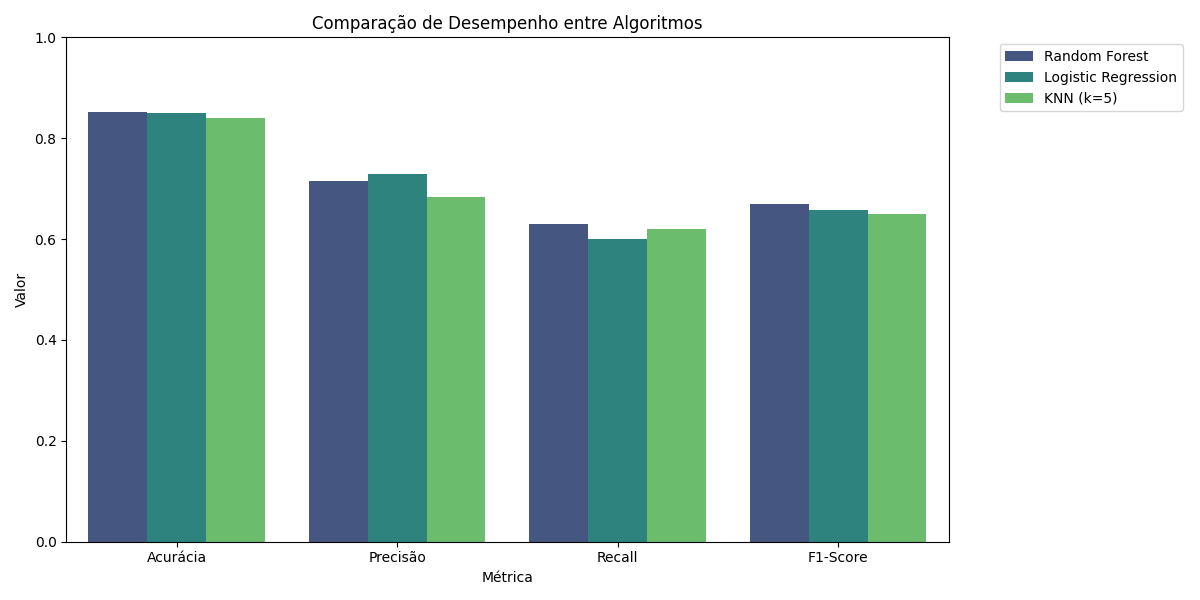
\includegraphics[width=0.78\textwidth]{../atividade_1/images/comparacao_desempenho.png}
    \caption{Comparação de desempenho entre os modelos avaliados.}
  \end{figure}
\end{slide}

\begin{slide}{Discussão e Conclusão}
  \begin{itemize}
    \item \textbf{Resumo:} pré-processamento adequado foi decisivo para a qualidade final.
    \item \textbf{Desafios:} limpeza de strings ruidosas evitou criação de classes duplicadas.
    \item \textbf{Conclusão:} a metodologia adotada permitiu análise crítica consistente dos modelos.
  \end{itemize}
\end{slide}

\begin{slide}{Referências}
  \begin{itemize}
    \item UCI Machine Learning Repository. Adult Census Income Dataset.
    \item Pedregosa et al. Scikit-learn: Machine Learning in Python.
    \item McKinney. Data Structures for Statistical Computing in Python (Pandas).
    \item Hunter. Matplotlib: A 2D Graphics Environment.
    \item Waskom. Seaborn: Statistical Data Visualization.
    \item Disciplina de Inteligência Computacional -- Prof. Dr. Alisson Marques da Silva.
  \end{itemize}
\end{slide}

\end{document}
